\subsection{Законы Кеплера}
\bfseries 1 закон: \mdseries  Все планеты движутся по эллиптическим орбитам, в одном из которых находится Солнце.(Рис. 2)
\begin{center}
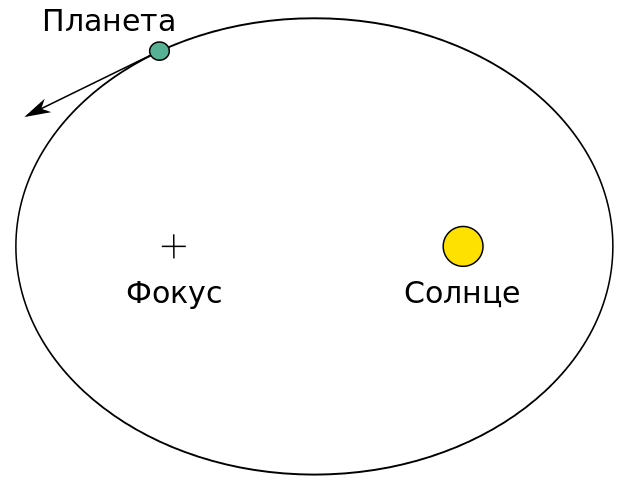
\includegraphics[scale=0.2]{First-Kepler's-law}
\begin{figure}[h!]
\caption {Первый закон Кеплера}
\end{figure}
\end{center}

\bfseries 2 закон: \mdseries Радиус-вектор планеты описывает за равные промежутки времени равные площади.(Рис. 3)
\begin{center}
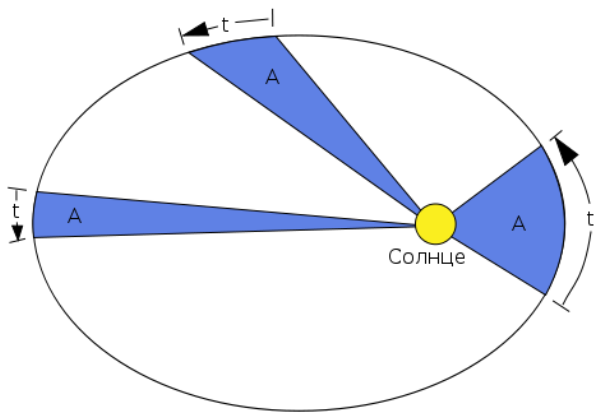
\includegraphics[scale=0.4]{Second-Kepler's-law}
\begin{figure}[h!]
\caption {Второй закон кеплера}
\end{figure}
\end{center}$$\frac{dS}{dt}=const$$
\bfseries 3 закон: \mdseries Квадраты периодов обращения планет относятся, как кубы больших полуосей их орбит.
$$\frac{T^2_1}{T^2_2}=\frac{a^3_1}{a^3_2}$$
Где $a$ --- большая полуось, $T$ --- период обращения.
Обобщённый Ньютоном 3 закон имеет слейдующий вид:
$$\frac{T^2_1(M+m_1)}{T^2_2(M+m_2)}=\frac{a^3_1}{a^3_2} \text{ или } \frac{T^2}{a^3}=\frac{4\pi^2}{G(M+m)}$$
Где $M$ --- масса центрального тела, $m_1$ и $m_2$ --- массы обращающихся тел. Так как массы планет m много меньше массы звезды $M$, то $M+m\approx M$